\documentclass{article}

\usepackage[margin=1in]{geometry}
\usepackage{amssymb, amssymb, amsthm}
\usepackage{enumitem}
\usepackage{courier}
\usepackage{listings}
\usepackage{graphicx}
\usepackage{fancyvrb}
\usepackage{color}
\usepackage{hyperref}

\definecolor{bgcolor}{rgb}{0.9, 0.9, 0.9}
\definecolor{light}{rgb}{0.5, 0.5, 0.5}
\def\light#1{{\color{light}#1}}

\lstset
{
    language=Python,
    numbers=left,
    stepnumber=1,
    showstringspaces=false,
    tabsize=4,
    breaklines=true,
    breakatwhitespace=false,
}

\begin{document}
\pagenumbering{gobble}

\begin{flushright}
Keegan Dahm \\
W207 \\
Lab 2
\end{flushright}

All my source files are at \href{https://github.com/TehVulpes/W207-Lab-2}{https://github.com/TehVulpes/W207-Lab-2}.

\begin{enumerate}[start=1]
\item % 1
    See the documents printouts in the ipynb PDF.
    
\item % 2
    My code has the following output:
    
    \begin{Verbatim}
Making basic vectorizer...
    In the training data, the total vocabulary is 26879 words
    The average non-zero matrix entries per sample is 96.70599803343165
    The fraction of non-zero / total matrix items is 196700 / 54671886, or
            0.0035978272269590263
    The 0th feature is "00", and the last is "zyxel"

Making vectorizer with limited vocabulary...
    The vocabulary of the new dataset is ['atheism', 'graphics', 'space',
            'religion']
    The average number of nonzero features per sample is 0.26843657817109146

Making vectorizer for character [2, 3]-grams...
    The vocabulary size of the new dataset is 35478

Making vectorizer that prunes words showing up in <10 documents...
    The vocabulary size of the new dataset is 3064

Checking for words in the dev dataset missing in the training dataset...
    Of the 16246 words in the dev vocab, 4027 are not in the training set.
    \end{Verbatim}
    
\newpage
    
\item % 3
    KNN doesn't work well for this type of problem because of how many features / dimensions the dataset has. KNN seems to work better with well-clustered data, and not with data scattered around the periphery. My code produced the following tables:
    
    \begin{Verbatim}
K Nearest Neighbors
    k = 1:  f-1 score: 0.3805030018531525
    k = 3:  f-1 score: 0.4084150225437623
    k = 5:  f-1 score: 0.4287607236218357
    k = 7:  f-1 score: 0.45047910006117586
    k = 9:  f-1 score: 0.4365666176198027
    k = 11: f-1 score: 0.4266108018696209

Naive Bayes
    a = 0.001:  f-1 score: 0.7702518836155706
    a = 0.01:   f-1 score: 0.7751663218544357
    a = 0.1:    f-1 score: 0.7903052385098862
    a = 1:      f-1 score: 0.7777320236017224
    a = 10:     f-1 score: 0.6674814338256576
    a = 100:    f-1 score: 0.5100896536573467
    a = 1000:   f-1 score: 0.3146996158261945
    
Logistic Regression
    C = 0.001:  f-1 score: 0.6193046812006844
        Sum sq weights: alt.atheism:    0.16509,comp.graphics:      0.20095,
                        sci.space:      0.18067,talk.religion.misc: 0.18724
                        
    C = 0.01:   f-1 score: 0.6646997417582748
        Sum sq weights: alt.atheism:    2.5415, comp.graphics:      2.9397,
                        sci.space:      2.8625, talk.religion.misc: 2.25
                        
    C = 0.1:    f-1 score: 0.6966243542418833
        Sum sq weights: alt.atheism:    27.132, comp.graphics:      24.663,
                        sci.space:      27.458, talk.religion.misc: 23.025
                        
    C = 1:      f-1 score: 0.6944172871853819
        Sum sq weights: alt.atheism:    166.98, comp.graphics:      130.93,
                        sci.space:      158.02, talk.religion.misc: 145.78
                        
    C = 10:     f-1 score: 0.6865669233056786
        Sum sq weights: alt.atheism:    585.26, comp.graphics:      448.03,
                        sci.space:      539.63, talk.religion.misc: 530.68
                        
    C = 100:    f-1 score: 0.6823892102438561
        Sum sq weights: alt.atheism:    1409.4, comp.graphics:      1082.3,
                        sci.space:      1284.4, talk.religion.misc: 1324.1
                        
    C = 1000:   f-1 score: 0.6787813199733858
        Sum sq weights: alt.atheism:    1913.5, comp.graphics:      1927.8,
                        sci.space:      2167.5, talk.religion.misc: 2451.5
    \end{Verbatim}
    
    Linear Regression performed worse than Naive Bayes because the labels for this data are descriptive, not numeric. NB is able to learn categorical relationships between features that Linear Regression has trouble with.
    
    The sum of squared weights seems to increase roughly linearly with C.
    
\newpage

\item % 4
    I'm including the table my code generated below. I noticed that "cheers kent" was the second strongest \texttt{alt.atheism} indicator. Looking in the dataset, it looks like Kent is very active in the \texttt{alt.atheism} newsgroup. Picking up on that might be overfitting, and might need manual tweaking to fix. Beside that, I noticed that \texttt{alt.atheism} had more varied ideological discussion, \texttt{talk.religion.misc} was mostly focused on Christianity, and the tone of religious language was a strong indicator between religion and atheism. The space and computer graphics newsgroups mostly stayed on topic, and their key indicators were domain-specific words.

    One thing I noticed in all of them are that there are seemingly low-information pairs of words, like "you are", "to my", "one of", or "out the".
    
    \begin{Verbatim}
alt.atheism       comp.graphics      sci.space           talk.religion.misc  
===========================================================================
claim that        looking for        the space           the fbi             
cheers kent       in advance         the moon            cheers kent         
was just          comp graphics      sci space           ignorance is        
you are           out there          and such            but he              
are you           is there           it was              of jesus            
in this           the image          the shuttle         off of              
the faq           thanks in          space station       is strength         
is not            know of            one of              the lord            
you ve            any help           of space            the word            
the motto         file is            in space            you were            
to say            to my              why not             with you            
you don           the screen         rather than         be with             
look up           version of         used to             such lunacy         
of islam          use the            nasa gov            teachings of        
notion of         24 bit             to see              the teachings       
of religion       does anyone        few years           compuserve com      
re right          and it             sherzer methodology may be              
natural morality  computer graphics  the spacecraft      out the             
an atheist        how to             sounds like         how about           
bake timmons      would like         the sun             objective morality  
    \end{Verbatim}

\item % 5
    For this, I found the following steps (in order) to be helpful:
    
    \begin{enumerate}[label=\arabic*.]
    \item Convert to lower case
    \item Remove quotes from contractions (e.g. ``you're'' $\rightarrow$ ``youre'')
    \item Replace any strings of numbers with the tag \texttt{INT}
    \item Replace all \texttt{INT.INT} sequences with the tag \texttt{FLOAT}
    \item Remove common 2 letter words (like ``of'', ``to'', ``in'', etc.), and ``the''
    \item Remove repeated symbols common in user signatures
    \item Replace repeated exclamation points with just a single one
    \item Remove the filler words ``very'' and ``extremely''
    \item Remove instances of the substring ``ation''
    \item Split sentence-ending punctuation to reduce vocabular (e.g. ``\texttt{done.}'' $\rightarrow$ ``\texttt{done .}'')
    \end{enumerate}
    
    Running it in my code had the following output:
    
    \begin{Verbatim}
Basic fitness:  0.7084739776490449  vocab size: 26879
Custom fitness: 0.7339321018867501  vocab size: 24981
The vocabulary changed by -1898 words
    \end{Verbatim}

\newpage

\item % 6
    The Linear Regression model's performance plateaued as the log of the vocabulary size increased. Below are the raw performance metrics and a graph:
    
    \begin{Verbatim}
L1 C=0.001, vocab size = 2 words,     with an f1 score of 0.3225085906291073
L1 C=0.01,  vocab size = 18 words,    with an f1 score of 0.4640942031795805
L1 C=0.1,   vocab size = 221 words,   with an f1 score of 0.6900662448603364
L1 C=0.5,   vocab size = 739 words,   with an f1 score of 0.6662891983103824
L1 C=0.7,   vocab size = 931 words,   with an f1 score of 0.6718820622771383
L1 C=0.9,   vocab size = 1081 words,  with an f1 score of 0.6852508594864148
L1 C=1,     vocab size = 1163 words,  with an f1 score of 0.6877600590884645
L1 C=10,    vocab size = 3576 words,  with an f1 score of 0.7019487752185992
L1 C=100,   vocab size = 7706 words,  with an f1 score of 0.7090742356994326
L1 C=1000,  vocab size = 24780 words, with an f1 score of 0.710072965652832
L1 C=10000, vocab size = 26854 words, with an f1 score of 0.710072965652832
L1 C=100000,vocab size = 26877 words, with an f1 score of 0.7084739776490449
    \end{Verbatim}
    
    \begin{center}
    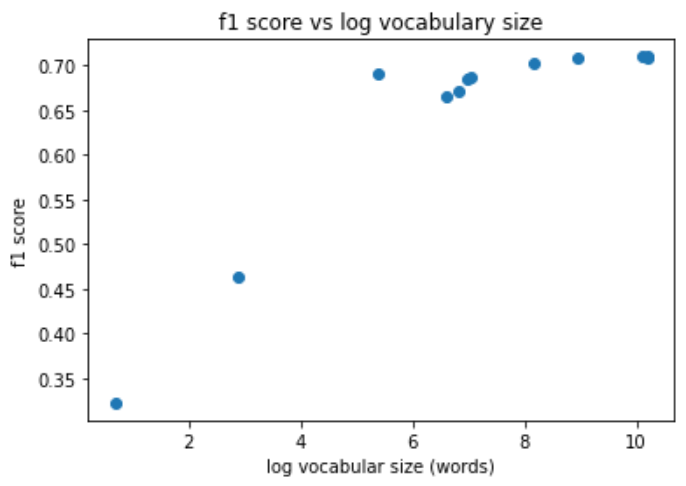
\includegraphics[width=13cm]{graph.png}
    \end{center}

\newpage

\item % 7
    \texttt{TfidfVectorizer} uses TF-IDF rather than count vectorization. It weighs unusually frequent words more heavily, so if a certain word is significantly more common in one document than in most others, it gives a lot of weight to that one word. The TF-IDF vectorizer's f1 score on my data set is 0.7597662427.

    The R ratio describes how "confidently incorrect" the classifier is. A high score here means the correct label got a low score, and an incorrect label got a high score. It seems to be applied to unusual discussion in each newsgroup. One method of improving this is to remove vocabular words that appear in *only* one label, which can be too weighty.
    
    My code produced the following output (snipped for brevity)
    
    \begin{Verbatim}
========================================
R = 929.3571373334202, label = talk.religion.misc, predicted = comp.graphics
========================================
I am pleased to announce that a *revised version* of _The Easy-to-Read Book
of Mormon_ (former title: _Mormon's Book_) by Lynn Matthews Anderson is now
available through anonymous ftp (see information below). In addition to the
change in title, the revised ETR BOM has been shortened by several pages
<snip>

As with the previous announcement, readers are reminded that this is a
not-for-profit endeavor. This is a copyrighted work, but people are welcome
to make *verbatim* copies for personal use. People can recuperate the
<snip>

FTP information: connect via anonymous ftp to carnot.itc.cmu.edu, then "cd
pub" (you won't see anything at all until you do).

"The Easy-to-Read Book of Mormon" is currently available in postscript and
RTF (rich text format). (ASCII, LaTeX, and other versions can be made
available; contact dba@andrew.cmu.edu for details.) You should be able to
print the postscript file on any postscript printer (such as an Apple
Laserwriter); let dba know if you have any difficulties. (The postscript in
the last release had problems on some printers; this time it should work
better.) RTF is a standard document interchange format that can be read in
by a number of word processors, including Microsoft Word for both the
Macintosh and Windows. If you don't have a postscript printer, you may be
able to use the RTF file to print out a copy of the book.

-r--r--r--  1 dba                   1984742 Apr 27 13:12 etrbom.ps
-r--r--r--  1 dba                   1209071 Apr 27 13:13 etrbom.rtf
<snip>

========================================
R = 325.0038462992751, label = talk.religion.misc, predicted = comp.graphics
========================================
Can anyone provide me a ftp site where I can obtain a online version
of the Book of Mormon. Please email the internet address if possible.

========================================
R = 287.3072077917014, label = alt.atheism, predicted = talk.religion.misc
========================================

The 24 children were, of course, killed by a lone gunman in a second story
window, who fired eight bullets in the space of two seconds...
    \end{Verbatim}


\end{enumerate}

\end{document}
